%%%%%%%%%%%%%%%%%%%%%%%%%%%%%%%%%%%%%%%%%
% University/School Laboratory Report
% LaTeX Template
% Version 3.1 (25/3/14)
%
% This template has been downloaded from:
% http://www.LaTeXTemplates.com
%
% Original author:
% Linux and Unix Users Group at Virginia Tech Wiki 
% (https://vtluug.org/wiki/Example_LaTeX_chem_lab_report)
%
% License:
% CC BY-NC-SA 3.0 (http://creativecommons.org/licenses/by-nc-sa/3.0/)
%
%%%%%%%%%%%%%%%%%%%%%%%%%%%%%%%%%%%%%%%%%

%----------------------------------------------------------------------------------------
%	PACKAGES AND DOCUMENT CONFIGURATIONS
%----------------------------------------------------------------------------------------

\documentclass{article}

\usepackage{graphicx} % Required for the inclusion of images
\usepackage{natbib} % Required to change bibliography style to APA
\usepackage{amsmath} % Required for some math elements 

\setlength\parindent{0pt} % Removes all indentation from paragraphs

\renewcommand{\labelenumi}{\alph{enumi}.} % Make numbering in the enumerate environment by letter rather than number (e.g. section 6)



\usepackage{geometry}
 \geometry{
 a4paper,
 total={170mm,257mm},
 left=20mm,
 top=20mm,
 }



%\usepackage{times} % Uncomment to use the Times New Roman font

%----------------------------------------------------------------------------------------
%	DOCUMENT INFORMATION
%----------------------------------------------------------------------------------------

\title{Introduction to Machine Learning:\\ Project assignment} % Title

\author{Fares \textsc{Meghdouri}} % Author name

\date{\today} % Date for the report

\begin{document}

\maketitle % Insert the title, author and date

\begin{center}
\begin{tabular}{l r}
Instructor: Prof. Dr. Dipl. Eng. Aggelos
Pikrakis % Instructor/supervisor
\end{tabular}
\end{center}

% If you wish to include an abstract, uncomment the lines below
% \begin{abstract}
% Abstract text
% \end{abstract}

%----------------------------------------------------------------------------------------
%	SECTION 1
%----------------------------------------------------------------------------------------

\section{Problem Statement}
In this homework, we try to build a set of classifiers (Naive Bayes, k-NN, Least-Squares-based, ANN and SVM) in order to predict a label of a collection of youtube videos from a well know set of labels. Since the raw video representation (frame-by-frame) is hard to deal with, the data is represented in our case in a special manner that will be discussed later. Once the classifiers are designed, a comparative study is to be done by evaluating each classifier using supervised learning metrics and connclude which is the best.

A cross-validation step is required to ensure the generalization of out approach. The final evaluation then consists of a 5-fold cross-validation in addition to a validation set that is, in our experiments, considered as a test set.


\section{Background}
We first start with the basics of each classifier that is used in this work. It is worth to mention that each of the following classifiers is based on a different approach of separation or predicting classes. The details provided here are superficial however, we refer the reader to the papers and articles referenced for more details.

\subsection{Bayesian Classifiers}
Bayesian classifiers are probabilistic classifiers based on the bayesian theorem. Under the assumption that input features are uncorrelated, the class of a test simple is predicted based on its conditionnal probability. Let us assume a data point $x$ such as $x = (x{1},...,x_{n})$ where $n$ is the number of features. A bayesian classifier will predict a class $C_{l}$ such as $p(C_{l})|x)$ is maximized. 

\subsection{k-Nearest Neighbors}

\subsection{Least Squares}

\subsection{Artificial Neural Networks}

\subsection{Support Vector Machines}

\subsection{Random Forests}

\section{Dataset Preprocessing}
An important step in any Machine Learning (ML) application is the data preprocessing. In fact, the representation and authenticity of the data is considered as a key characteristic that decide weather further operation will be successful or not. That is the reason why we invested time and resources cleaning the data as good as possible. We use the Youtube-8M dataset in this work \cite{} that is know to be a huge datasets of labeled youtube videos (~ 8 million videos). 
% talk about how they labeled it
We use the \emph{Video-level features dataset} which is a version of the dataset that consists of two sets of features in addition to a label. The first set of features are audio features consisting of 128 real values feature extracted using ... . The second set of features are the video features consisting of 1024 real valued features. We get a total of 1152 features which is at a first glance a massive number with wich we assume that most ML algorithms will either take forever to train or overfit if the amount of data is not enough.

We moreover, select only three classes from the dataset instead of the whole 3862 classes. By trial and error (with the goal of maximizing performance) we opted for the followinf classes: sdsa,asdasd and asdsa. Table \ref{} show the IDs and the cound of data simple in out sub-dataset.

\begin{table}
\center

\begin{tabular}{l*{6}{c}r}
ID           & label & \# instances in raw training set & Train set & Validation set \\
\hline
19 			 & Racing & 84258 & 84285 & 24182 \\
23          & Smartphone & 64884 & 64893  & 18726 \\
33          & Drum & 54195 & 54199 & 15705 \\

\end{tabular}
\caption{Dataset classes.}
\end{table}
% table goes here

\begin{figure}[!htb]
   \begin{minipage}{0.5\textwidth}
     \centering
     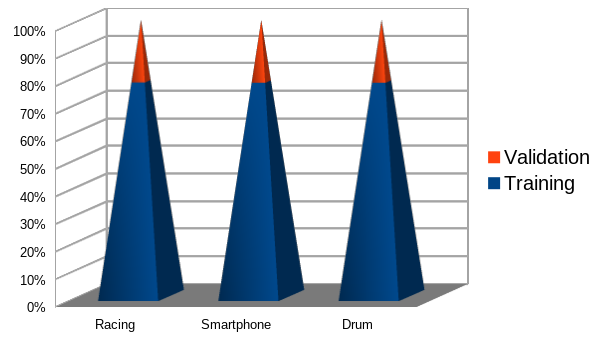
\includegraphics[width=\linewidth]{img/d_s}
     \caption{Interpolation for Data 1}\label{Fig:Data1}
   \end{minipage}\hfill
   \begin{minipage}{0.5\textwidth}
     \centering
     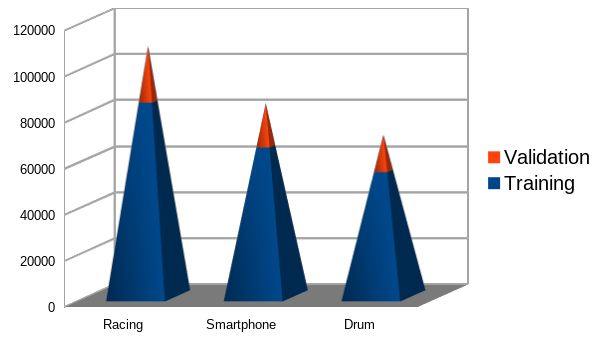
\includegraphics[width=\linewidth]{img/d}
     \caption{Interpolation for Data 2}\label{Fig:Data2}
   \end{minipage}
\end{figure}


In order to extract the previous features we go through all the tensorflow protocol buffer (which is a special representation of data to store in physicaly) and for each, we first extract the label and compare it into our suited list. If the former matches our choice, we parse the set of features and append them into a output file on the hard drive. The final representation of the data is a Comma Separated Values (CSV) containing 1152 features and a label. Files are eventually available publically\footnote{download me}.

In order to reduce dimentionnality, we opt for two techniques:
\begin{itemize}
\item We convert the original space into a rotated space by maximizing the variance in the first few dimentions. This can easily be achieved by Principal Compenent Analysis (PCA). After experiements, we noticed that the first 600 dimentions contributes 80\% to the representation of the data thus, we chose to sacrified 20\% of the information to reduce the dimentionality by 50\%. Figure \ref{fig:pca} show the accumulative variance distribution of all components.

\item In order to reduce the dimentionnality even further, however this time carefully, we apply DEcision Trees (DT) feature importance which is a metric for how pure a feature is (in other words, fetaures with hight split in the tree get higher importance). Applying this technique and removing features with vanishing importance let us reduce out space to xxx features. We note here that this technique does not preserve 100\% of the data as PCA did.
\end{itemize}

One of the decision we had to make here is the order of reduction. In order not to loose any information at the begining, we chose to perform first (lossless) PCA then apply DT feature importance.

It is worth to mention that ANNs are able to learn the feature importance without the previous steps however, if we aim for a fair comparison, all alggorithms need to be fed the same data and thus, we opt for a dimentionnality reduction to adapt the data to the majority of algorithms.

\begin{figure}
\center
  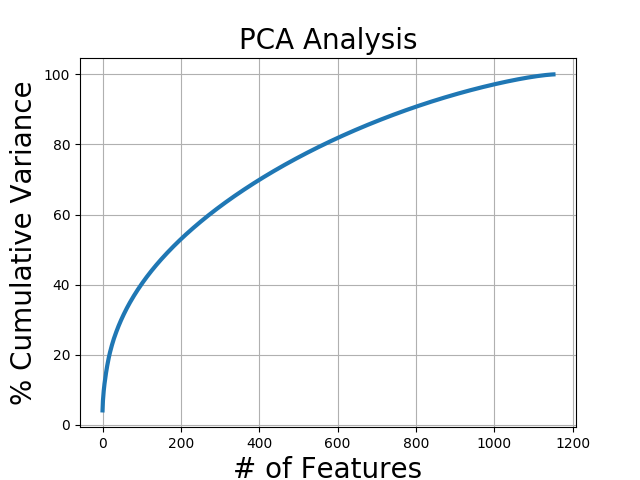
\includegraphics[width=0.5\linewidth]{img/PCA_Analysis}
  \caption{PCA analysis.}
  \label{fig:pca}
\end{figure}

\section{Experiments}



\section{Results and Disscussions}


\section{Conclusion}
%----------------------------------------------------------------------------------------
%	BIBLIOGRAPHY
%----------------------------------------------------------------------------------------

\bibliographystyle{apalike}

\bibliography{sample}

%----------------------------------------------------------------------------------------


\end{document}